%
% LAYOUT.TEX - Kurzbeschreibung von PA 88-10-04 (LaTeX)
%                                      99-03-20
%
%  Updated for REFMAN.CLS (LaTeX2e)
%
\documentclass[twoside,a4paper]{refart}
%\documentclass[pagesize,twoside,a5paper,smallborder,10pt]{refart}
\usepackage[T1]{fontenc}
\usepackage{ae} % CM-Zeichens"atze mit T1 encoding
\usepackage{makeidx}
\usepackage{ifthen}
\usepackage{german}
%\usepackage{showidx}
\usepackage[pdftex]{graphicx}
\usepackage{wrapfig}
\usepackage{hyperref}

\DeclareRobustCommand\cs[1]{\texttt{\char`\\#1}}
\def\bs{\char'134 } % backslash in \tt font.
\newcommand{\zB}{z.\,B.}
\newcommand{\dH}{d.\,h.}  

\title{Dieselpartikelfilter Austausch VW 2.0 TDI CAAB}
\author{TX-BOARD.de \\Nutzer 3pleL \\}

\date{}
\emergencystretch1em  % F"ur TeX <3.0 auskommentieren!

%\pagestyle{footings}
%\pagestyle{headings}
%\pagestyle{myfootings}
\markboth{Layout-"Anderungen mit \textrm{\LaTeX}}%
         {Layout-"Anderungen mit \textrm{\LaTeX}}

\makeindex % Dies nur als Demonstration, das jetzt auch ein Index
           % m"oglich ist :-)
% Bei Marginlabels mu"s der Index *vor* dem Label stehen.

% Es ist notwendig die Umlaute in der TeX-Schreibweise zu schreiben,
% da der german.sty sie sonst in etwas verwandeln w"urde, mit dem
% MakeIndex nicht zurecht kommt.


\setcounter{tocdepth}{2}
\settextfraction{0.7}

\begin{document}
\maketitle

\begin{abstract}
	Der vorliegende Erfahrungsbericht beschreibt den Wechsel des Dieselpartikelfilter (DPF) an einem VW T5 Facelift mit 2.0l TDI Dieselmotor (CAAB). Er basiert überwiegend auf verstreuten Posts hier im Forum, der original Reparaturanleitung und einigen YouTube Videos. Er ersetzt \textbf{NICHT} die originale Anleitung, die über \href{https://erwin.volkswagen.de/erwin/showHome.do}{Erwin} verfügbar ist. Auch ersetzt dieser Bericht nicht den gesunden Menschenverstand und sorgfältigstes Arbeiten. 
	Da ich kein ausgebildeter Mechaniker bin, betrachte man diesen Bericht nicht als der Weisheit letzten Schluss sondern lediglich als ergänzende Notizen!
\end{abstract}

\tableofcontents

\newpage


%%%%%%%%%%%%%%%%%%%%%%%%%%%%%%%%%%%%%%%%%%%%%%%%%%%%%%%%%%%%%%%%%%%%

\section{Einleitung}

\subsection{Benötigtes Werkzeug}
\begin{itemize}
	\item Wagenheber
	\item Unterstellböcke
	\item Rätschenkasten 
	\item Satz Maulschlüssel
	\item Schlauchschellenzange
	\item Winkelschleifer 
	\item Hammer
	\item Rostlöser/WD-40 o.ä.
	\item Bunsenbrenner o.ä.
	\item Licht
	\item VCDS
\end{itemize}

\subsection{Benötigte Ersatzteile}
\begin{itemize}
	\item Dieselpartikelfilter (DPF)
	\item Blechdichtung 1K0 253 115T (Turbo - DPF)
	\item Dichtung 7H0 253 115D (DPF - Flexrohr)
	\item 2x V-Bandschelle 1K0 253 725
\end{itemize}

\marginlabel{Kommentar:}
Die Schelle am Turbo konnte ich zerstörungsfrei demontieren und somit wiederverwenden.

\subsection{Video-Quellen}

\href{https://www.youtube.com/watch?v=Uml32Phw4O8}{VW T5 1.9 TDI DPF} - Sieht bei dem 1.9 ganz ähnlich aus, wie beim 2.0\\
\clearpage
\section{DPF ausbauen}
\marginlabel{Kommentar:}
Ein Helfer ist für das Aus- und wieder Einbauen des DPF sehr empfehlenswert (ich hätte es ohne Helfer nicht machen wollen)! 

\subsection{Im Motorraum}
\begin{enumerate}
\item Schelle am Turbo (Abb. \ref{fig:ubersicht} -3-) mit WD40 bearbeiten und lösen
\item Steckverbinder lösen (Abb. \ref{fig:motorraum}) und Kabelstrang bis zu den Sensoren freilegen 
\item Platz schaffen
    \begin{enumerate}
    \item Kühlmittelbehälter beiseite legen
    \item Ladeluftschlauch ggf. demontieren
    \end{enumerate}
\item Differenzdrucksensor (DDS) demontieren (Abb. \ref{fig:ubersicht} -15-)
\item Halter DDS Rohre lösen (Abb. \ref{fig:ubersicht} -22-)
\end{enumerate}
\begin{figure}[htb]
	\begin{center}
		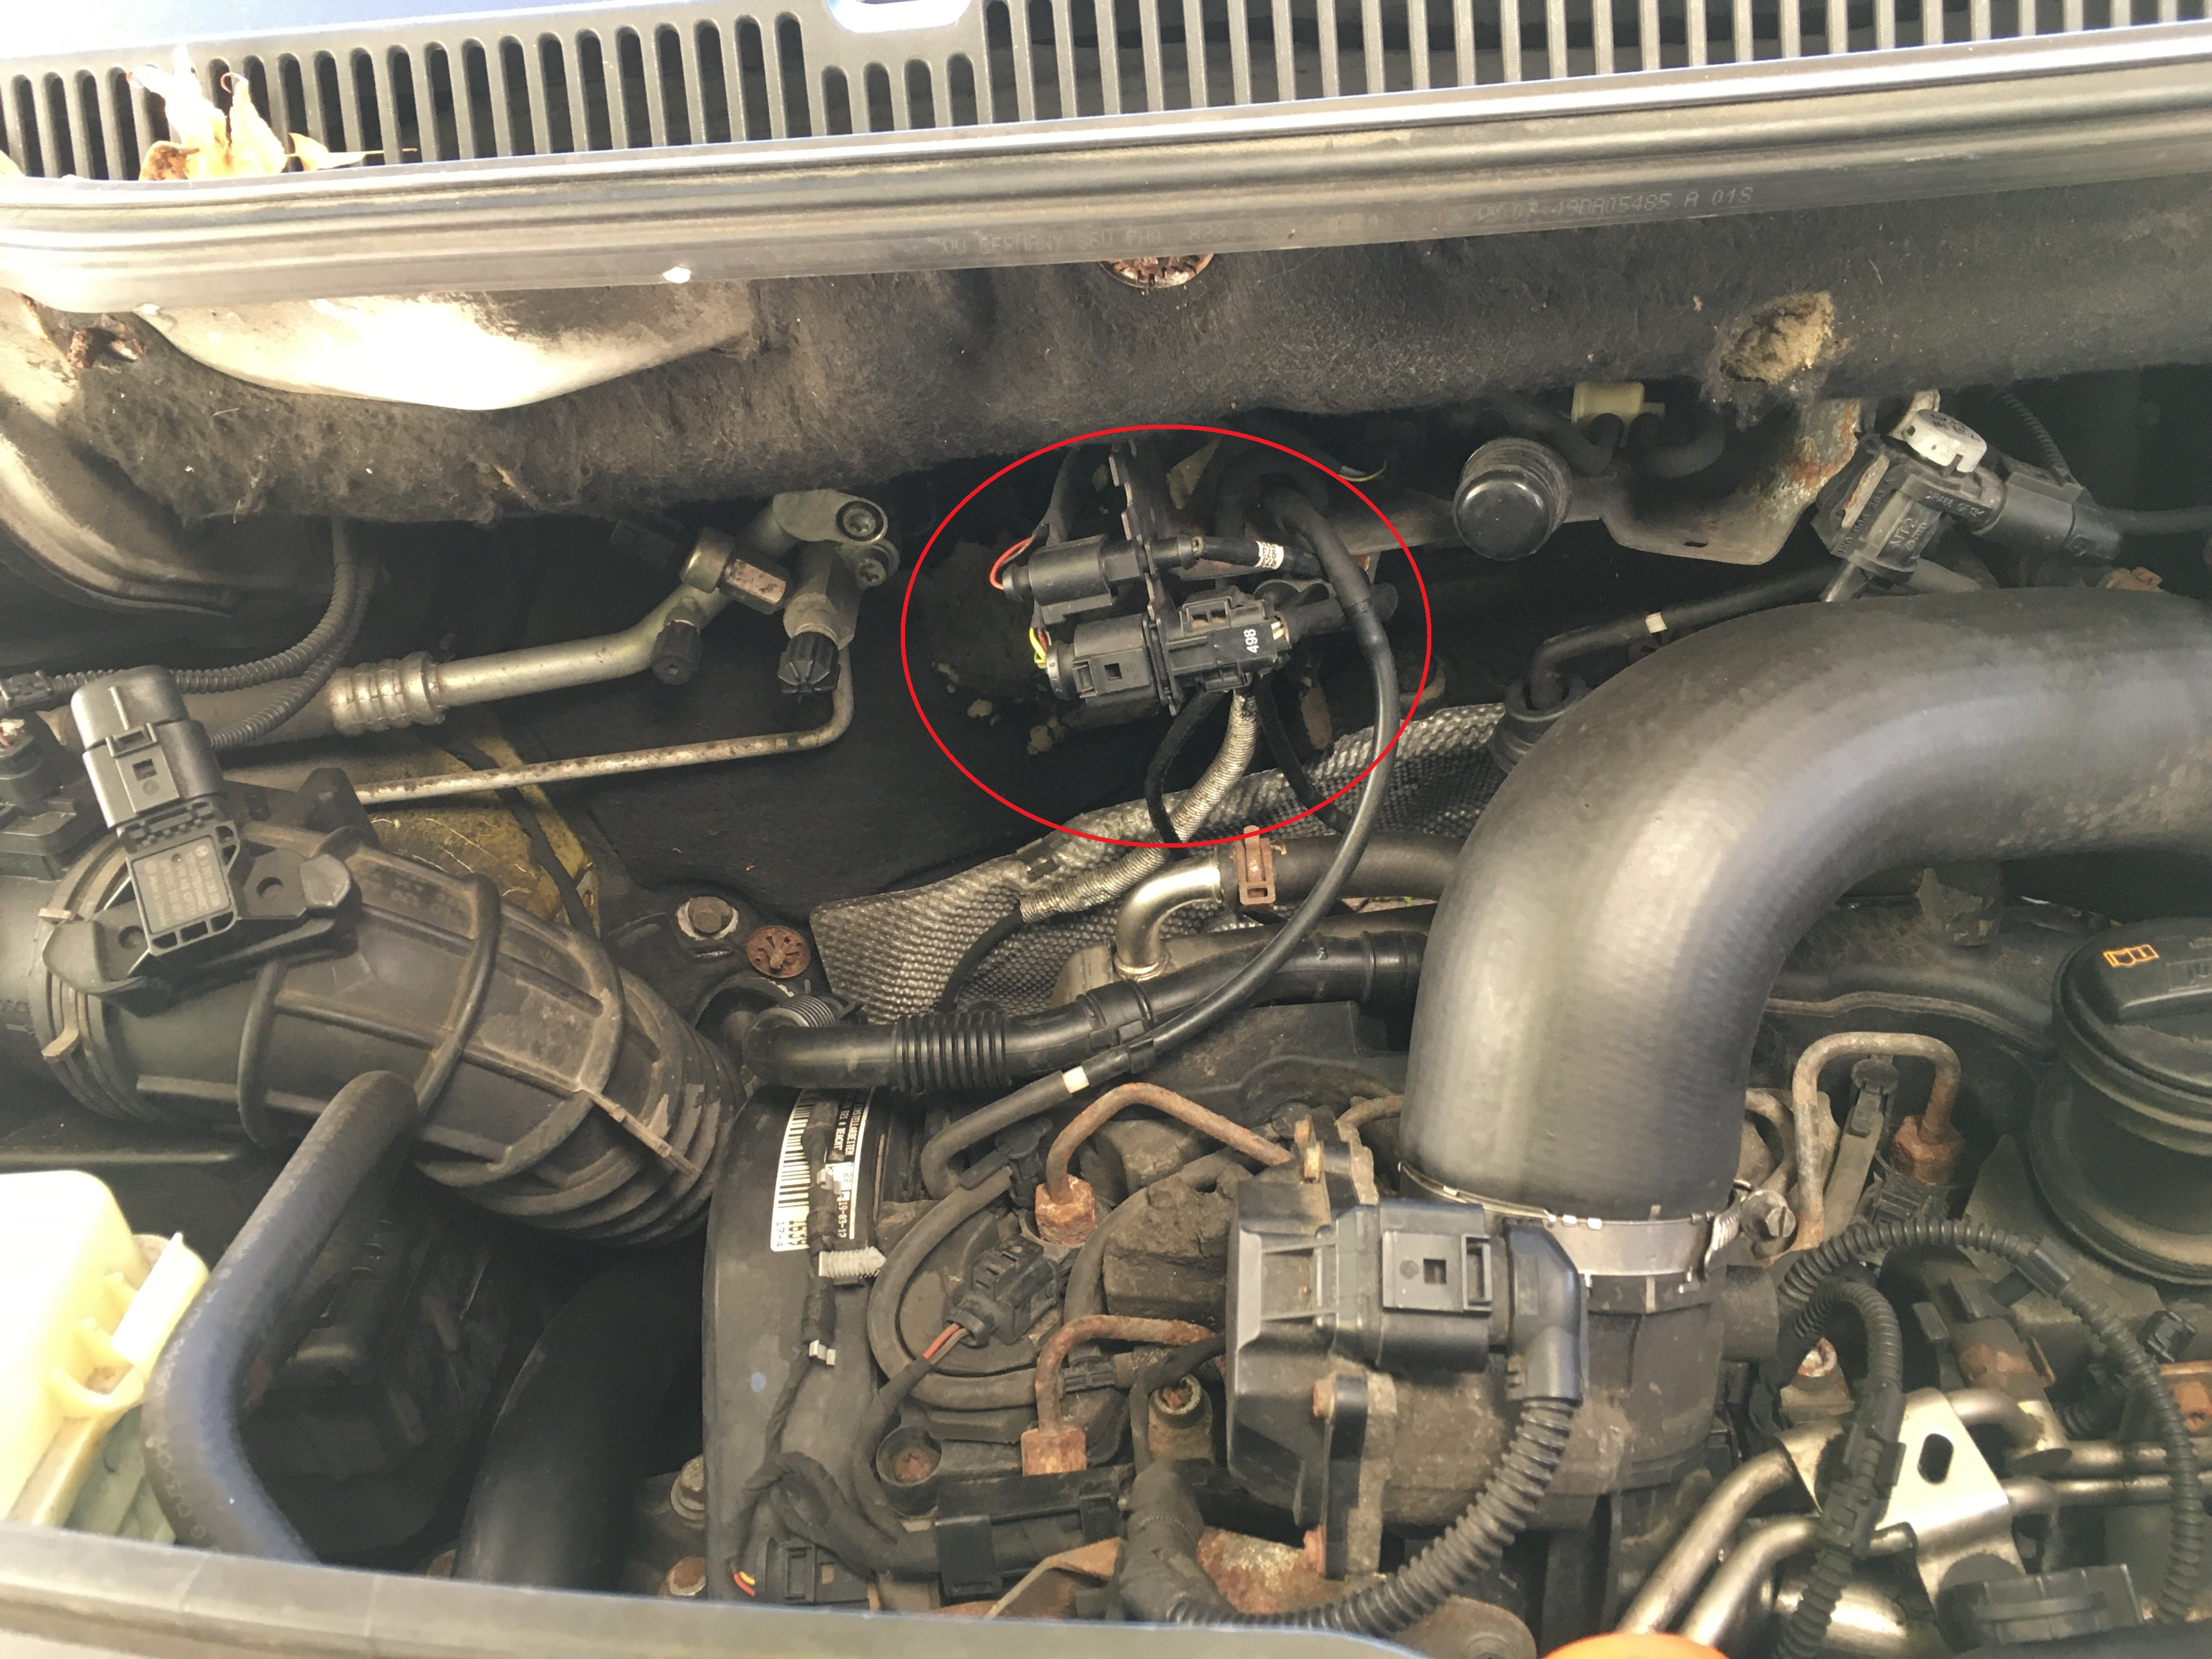
\includegraphics[width=\textwidth]{Motorraum.JPG}
		\caption{Stecker im Motorraum}
		\label{fig:motorraum}
	\end{center}
\end{figure}
\clearpage
\subsection{Unter dem Auto}
\begin{enumerate}
\item Schelle mit WD40 bearbeiten und lösen
\item Stecker Temperatursensor(braun) lösen
\item Schraube (Abb. \ref{fig:ubersicht} -8-) und Muttern (Abb. \ref{fig:ubersicht} -7/9-) lösen
\item DPF herausnehmen
\end{enumerate}
\begin{figure}[htb]
	\begin{center}
		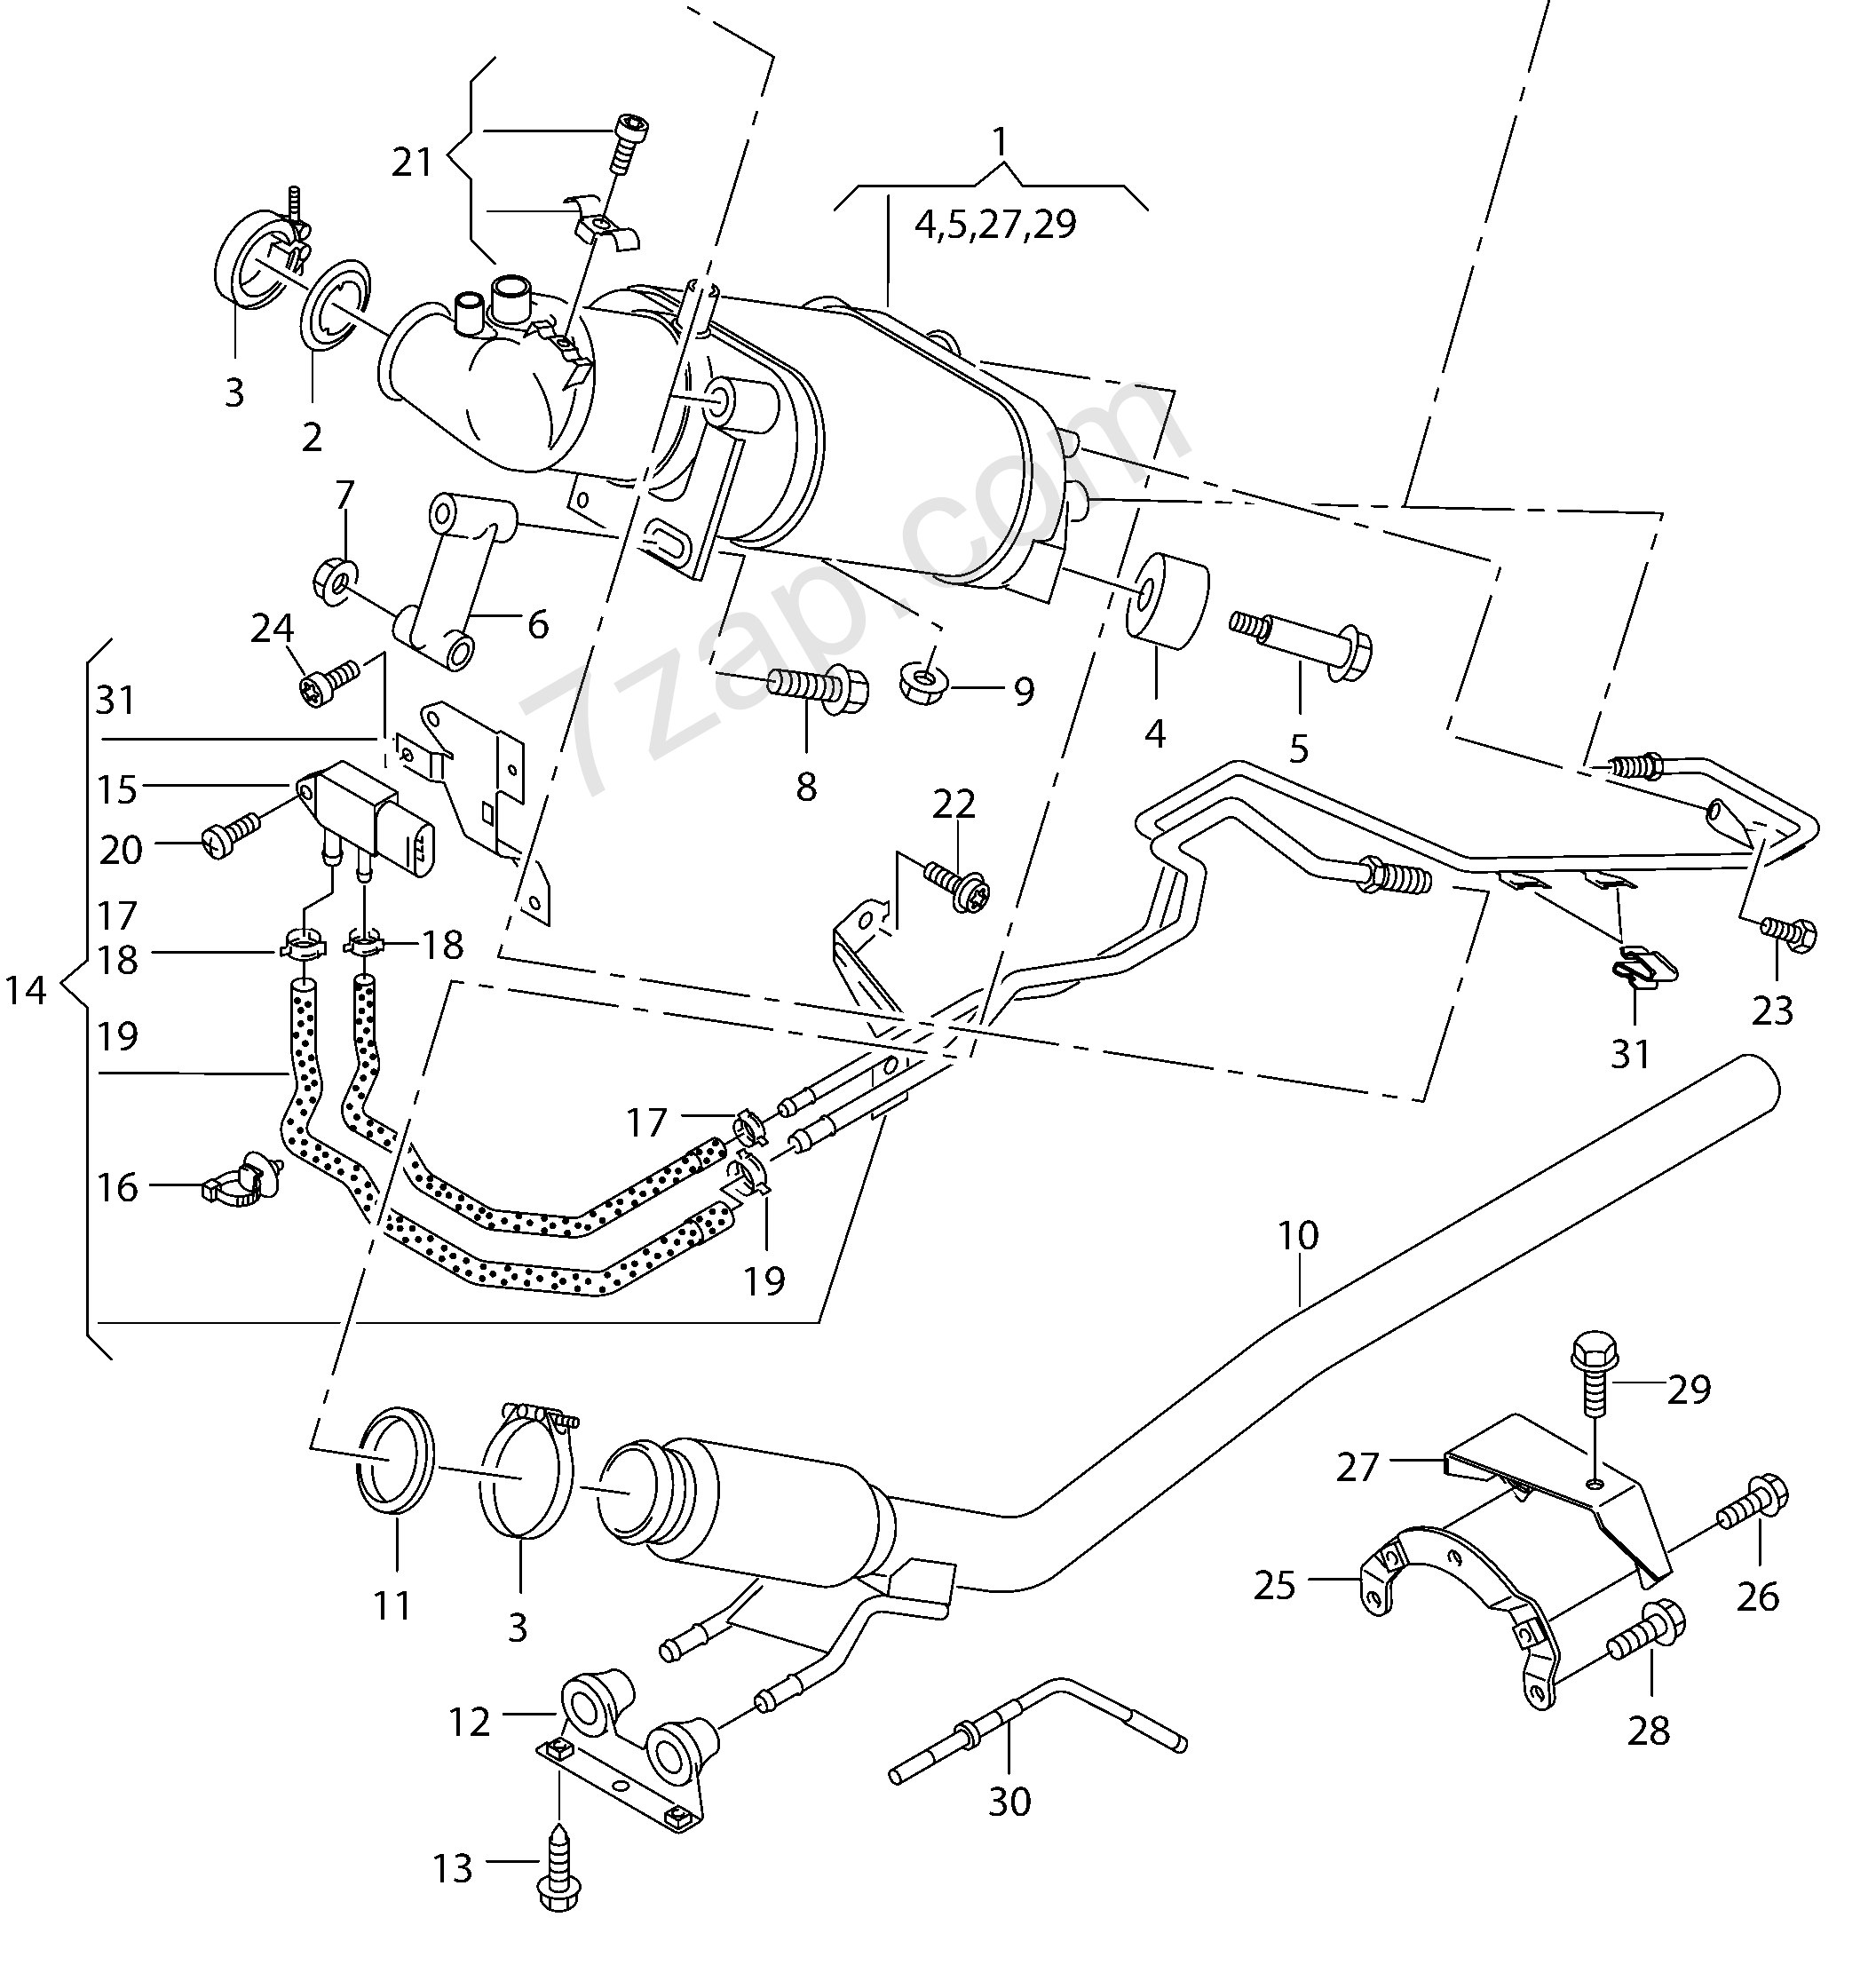
\includegraphics[width=\textwidth]{UbersichtDPF}
		\caption{Übersicht DPF}
		\label{fig:ubersicht}
	\end{center}
\end{figure}
\marginlabel{Kommentar:}
Die Dichtung (Abb. \ref{fig:ubersicht} -11-) und Schelle zum Flexrohr waren bei mir sehr stark mit allen Komponenten verbacken. Die Schraube der Schelle lies sich zwar leicht öffnen aber danach bewegte sich nichts. Deshalb habe ich mit dem Winkelschleifer das Metallband der Schelle durchtrennt und an dieser Stelle einen Schraubendreher eingetrieben um so die Schelle zu lösen. Die Dichtung lies sich auch nur mit viel Geduld und fleißigem Stochern mit einer Messerklinge vom Flansch des Flexrohr entfernen. Insgesamt waren dies die unangenehmsten Arbeiten bei der gesamten Aktion.
\newpage

\section{Sensoren ausbauen}
Einer der Temperatursensoren ließ sich in meinem Fall einfach mit dem Maulschlüssel lösen, die Lambdasonde braucht ein paar zarte Schläge mit dem Hammer auf den Schlüssel um sich zu bewegen. Der zweite Sensor saß sehr fest. Nach Erhitzen der Mutter am DPF mit einem kleinen Brenner ließ dieser sich auch lösen.

Die Druckschläuche zum DDS saßen auch recht fest, weshalb ich diese erst nach Ausbau des DPF gelöst habe (entgegen der Anleitung, dies schon vorher zu tun).

\section{Sensoren einbauen}
Die Sensoren müssen mit Heißschraubenpaste (in meinem Fall Liqui Moly Keramikpaste) eingesetzt werden. Dabei darauf achten, nur das Gewinde zu schmieren und nicht den Sensor. Theoretisch wird die Lambdasonde mit 50Nm festgezogen, die Temperatursensoren mit 45Nm.

Die Schläuche zum DDS habe ich auch vor Einbau montiert, das Aufstecken der Schläuche im beengten Motorraum erscheint mir wenig sinnvoll.

\section{DPF einbauen}
Beim Einbau des DPF ist wieder ein Helfer sinnvoll, der vom Motorraum aus dirigieren und die DDS Leitungen führen kann.

Um einen spannungsfreien Einbau zu gewährleisten folgende Reihenfolge bei der Montage beachten:
\begin{enumerate}
	\item Mutter (Abb. \ref{fig:ubersicht} -7-) muss lose sein und den Filter mit der Schraube (Abb. \ref{fig:ubersicht} -8-) lose befestigen
	\item DPF am Turbo ansetzen (Dichtung nicht vergessen) und die Schelle festziehen
	\item Mutter an der Drehmomentstütze festziehen (40Nm)
	\item Schraube (Abb. \ref{fig:ubersicht} -8-) festziehen (40Nm)
	\item Mutter (Abb. \ref{fig:ubersicht} -7-) festziehen (40Nm)
\end{enumerate}

Im Anschluss das Flexrohr mit Dichtung und Schelle am DPF befestigen.
Danach nur noch die Stecker einstecken und die Änderungen im Motorraum rückgängig machen.

\marginlabel{Kommentar:} Das Ansetzen des DPF am Turbo hat einige Versuche gebraucht, hier nicht die Geduld verlieren ;)
\section{VCDS}
Dem Motorsteuergerät muss im Anschluss an den Austausch noch der neue Filter bekannt gemacht werden. Dazu gibt es im Motorsteuergerät die Anpassungsfunktion \textbf{IDE00275 - Initialisierung des Partikelfilters}. Dieser Funktion wird der km-Stand des Partikelfilters in tausend-km übergeben. 

Ein Zugriff ist allerdings nur mit Login Code möglich.
In meinem Fall wurde von VCDS 27971 vorgeschlagen und auch akzeptiert, jedoch kam immer wieder die Meldung mit dem Zugriffscode. Der korrekte Code war \textbf{12233}.

Zusätzlich kann es sinnvoll sein eine (erzwungene) Regenerationsfahrt zu machen, um die Rußbeladung zurückzusetzen. Da jedoch meine letzte Regeneration 15km vor dem Austausch war habe ich mir dies gespart.

\section{Gereinigt oder Neu?}
Da der DPF eine sensible Baugruppe zu sein scheint und die Suche im Forum sehr gemischte Ergebnisse für die unterschiedlichen Lösungen brachte, habe ich mich dazu entschlossen den Filter bei der Firma Barten reinigen zu lassen.

Diese meldeten sich bei mir mit der Nachricht von einem Haarriss ausgangsseitig im Monolith. Wohl ein häufiger Defekt aber ohne Garantie haben sie mir den Filter dennoch gereinigt.

Nach guten 1000km hat sich das Regenerationsintervall wieder angehoben und ich bin bislang zufrieden. Das Regenerationsverhalten werde ich weiterhin beobachten und mich melden, sollte sich daran etwas ändern.

%%%%%%%%%%%%%%%%%%%%%%%%%%%%%%%%%%%%%%%%%%%%%%%%%%%%%%%%%%%%%%%%%%%%%%

\printindex

\end{document}
